\setchapterimage{west_div_roux_cropped}
\setchapterpreamble[u]{\margintoc}
\chapter{Divertor inventory estimation}\label{Chapter4}\labch{Chapter4}
\labch{Divertor inventory estimation}

% \section{Introduction}

This Chapter focusses on the estimation of the H inventory in the divertors of WEST and ITER.
This estimation relies on the monoblock behaviour law computed in \refch{Chapter3}.
This behaviour law allows rapid evaluations of the monoblocks H inventory for any exposure condition.
Inputs are taken from SolEdge3X-EIRENE \cite{bufferand_three-dimensional_2019} and SOLPS-ITER \cite{kaveeva_solps-iter_2020} plasma simulations.
The influence of several control parameters is investigated: the input power (i.e.\ how much heating power is injected in the plasma), the gas puffing rate (used in most tokamaks to increase the plasma density \cite{zweben_effect_2014}), and the divertor pressure of neutral particles in ITER.


\section{Methodology}
To make use of the monoblock inventory behaviour law, distribution of surface concentrations and surface temperatures along the divertors will be required.
They will be converted from plasma simulations outputs.

\subsection{Plasma simulations}

\begin{figure}[h!]
    \centering
    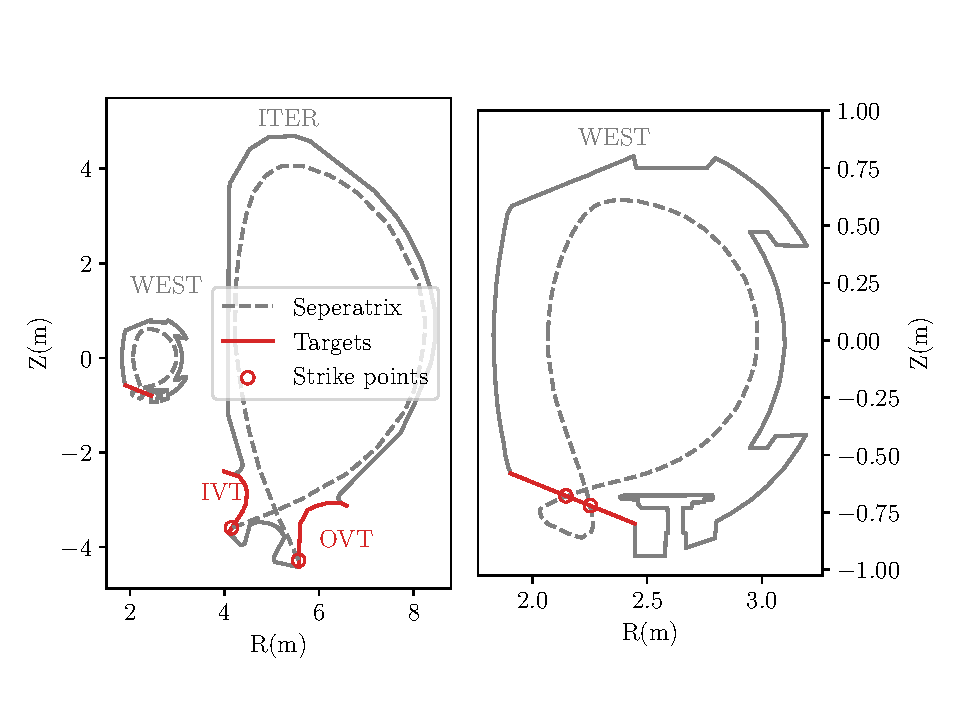
\includegraphics[width=0.95\linewidth]{Figures/Chapter4/coordinates.pdf}
    \caption{Geometry of WEST and ITER divertors.}
    \labfig{reactors}
\end{figure}
This Section describes the parameters of the plasma simulations.
These simulations were run with SolEdge3X-EIRENE for WEST and SOLPS-ITER for ITER.
In a nutshell, these codes solve, for each species (ions and electrons), the particle density, velocity and temperature.
The equations at stake are comparable to the Navier-Stokes equations coupled to the heat equation and interactions with the electromagnetic fields in the plasma \sidecite{bufferand_numerical_2015}.
Subsequently, the incident particle fluxes, heat fluxes and particle energy can be calculated along the tokamak wall.
For the SolEdge3X-EIRENE runs, the puffing rate and the input power were used as control parameters.
For SOLPS-ITER calculation, the divertor neutral pressure is the control parameter.

\subsubsection{SolEdge3X-EIRENE runs}
The Lower-Single-Null magnetic configuration used for the 2D simulations in SolEdge3X-EIRENE transport code (v588.165) are based on the experimental WEST plasma discharge \#54903 at $T_\mathrm{flat-top} = \SI{8}{s}$ (see \reffig{reactors}).
In order to get as many divertor conditions as possible, the puffing rate was varied from \SI{4.5e20}{molecule.s^{-1}} to \SI{4.72e21}{molecule.s^{-1}} and the input power from \SI{0.449}{MW} to \SI{2.5}{MW}.
The setup parameters of the simulation are listed in \reftab{my_tab}.
$R_\mathrm{wall}$ is the recycling coefficient of main chamber wall, $R_\mathrm{pump}$ is the recycling coefficient of the pump, $D$ is the cross-field mass diffusivity perpendicular to the flux surface, $\nu$ is the momentum diffusivity, $\chi_e$ and $\chi_i$ are the energy diffusivity for electrons and ions, respectively.
While the value of these coefficients is required for the sake of reproducibility, their detailed description is outside the scope of this research.
More information can be found in \sidecite{ciraolo_first_2019}.
The gas puff position is set inside the private region (i.e.\ the region between the two strike points) and the pump position is set under the baffle.

\begin{table}[!ht]
    \centering
    \caption{Setup parameters used in the SOLEDGE3X simulations.}
    \begin{tabular}{L{0.4\linewidth}  R{0.4\linewidth}}
    \hline \\
    Plasma composition & Deuterium, no impurity \\
    \\
    Recycling coefficients &  $R_\mathrm{wall} = 0.99$ \\
     & $R_\mathrm{pump} = 0.95$ \\
    \\
    SOL input power & from \SI{0.449}{MW} to \SI{2.5}{MW} \\
    \\
    Gas puffing rate & from \SI{4.5e20}{molecule.s^{-1}} to \SI{4.72e21}{molecule.s^{-1}} \\
    \\
    Drifts & - \\
    \\
    Transport coefficients & $D = \SI{0.3}{m^2.s^{-1}}$ \\
     & $\nu = \SI{0.3}{m^2.s^{-1}}$ \\
     & $\chi_e = \chi_i = \SI{1.0}{m^2.s^{-1}}$ \\
    \end{tabular}
    \labtab{my_tab}
\end{table}


\subsubsection{SOLPS runs}
Several ITER cases were taken from \sidecite{pitts_physics_2019} with divertor neutral pressures varying from \SI{1.8}{Pa} to \SI{11.2}{Pa}.
These SOLPS \sidecite{kaveeva_solps-iter_2020} scenarios can be found in the ITER Integrated Modelling Analysis Suite (IMAS) database \sidecite{imbeaux_design_2015, park_assessment_2020}.
The nine simulations used in this work are labelled 122396, 122397, 122398, 122399, 122400, 122401, 122402, 122403 and 122404.
These have been run in baseline burning plasma conditions ($Q=10$ with \SI{50}{MW} of input power).


\begin{figure}[h!]
    \centering
    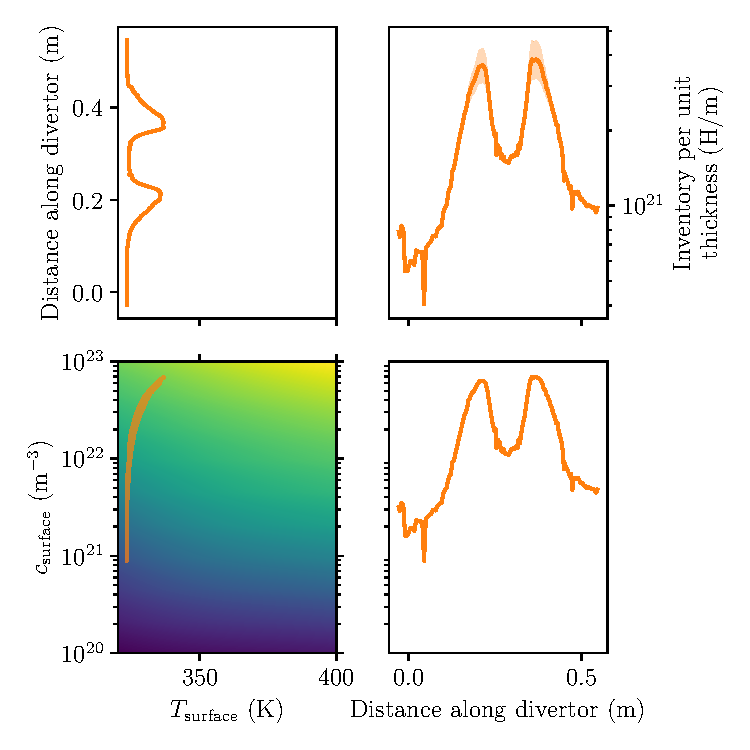
\includegraphics[width=\linewidth]{Figures/Chapter4/example.pdf}
    \caption{Method of divertor H inventory estimation based on the surface concentration, the surface temperature and the behaviour law obtained in \refch{Chapter3}.}
    \labfig{behaviour law example}
\end{figure}

\subsection{Estimation of exposure conditions}

\begin{figure*}[h]
    \centering
    \begin{subfigure}{0.5\linewidth}
        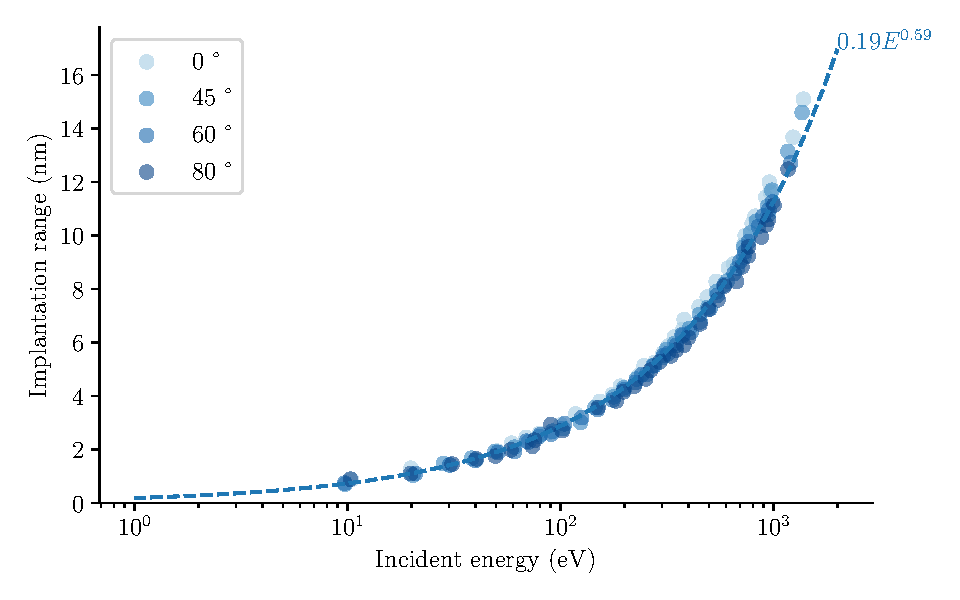
\includegraphics[width=\linewidth]{Figures/Chapter4/implantation_range.pdf}
        \caption{Implantation range $R_p$.}
        \labfig{implantation range vs energy}
    \end{subfigure}%
    \begin{subfigure}{0.5\linewidth}                          
        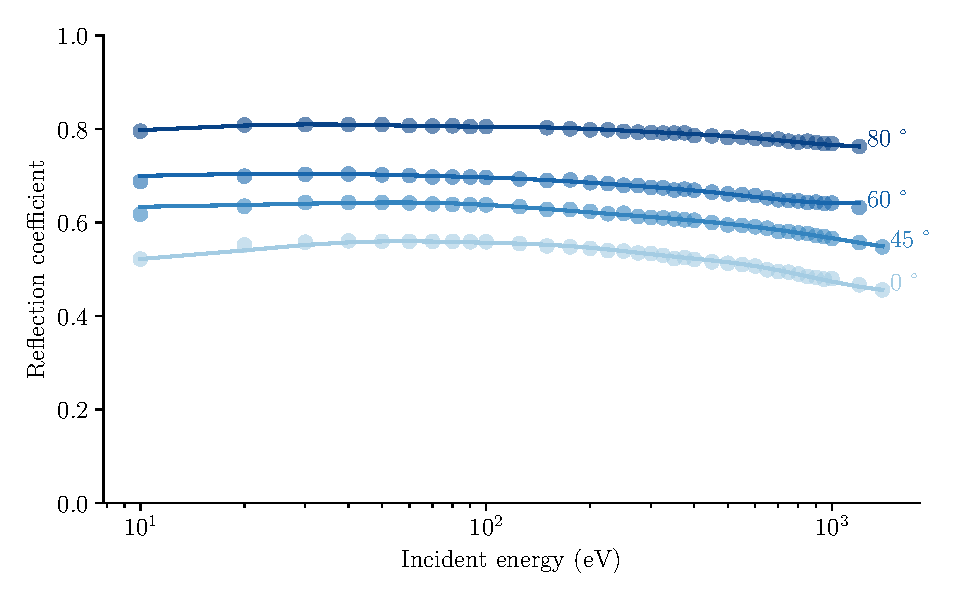
\includegraphics[width=\linewidth]{Figures/Chapter4/reflection_coeff.pdf}
        \caption{Reflection coefficient $r$.}
        \labfig{reflection coeff vs energy}
    \end{subfigure}
    \caption{Evolution of the implantation range and the reflection coefficient as a function of incident energy $E$ and angle of incidence.}
\end{figure*}

According to the behaviour law obtained in \refch{Chapter3}, the temporal evolution of the H inventory along the divertors can be estimated from the surface concentration of mobile hydrogen and surface temperature (see \reffig{behaviour law example}).
% This inventory distribution can then be projected onto the whole divertor geometry for better visualisation (see \reffig{top view}).

The distribution of the exposure conditions (angles of incidence, particles energies, particles fluxes and heat flux) are produced by SOLEDGE/SOLPS along the divertors of WEST and ITER (see \reffig{reactors} and \reffig{behaviour law example}).
These exposure conditions are converted into distributions of surface temperature $T_\mathrm{surface}$ and surface hydrogen concentration $c_\mathrm{surface}$ by \refeq{thermal behaviour law} and \refeq{c_surface}.

Note: see \refsec{monoblock thermal behaviour} for more details on the monoblock thermal behaviour.
\begin{equation}
    c_\mathrm{surface} = c_\mathrm{surface, \, ions} + c_\mathrm{surface, \, atoms}
    \labeq{c_surface}
\end{equation}
$c_\mathrm{surface, \, ions}$ and $c_\mathrm{surface, \, atoms}$ are the contributions of the ions and atoms to the surface hydrogen concentration.
They can be expressed as:
\begin{equation}
    c_\mathrm{surface, \, i} = \frac{R_{p, \mathrm{i}} \ \varphi_\mathrm{imp, \,i}}{D(T_\mathrm{surface})}
\end{equation}
where $R_{p, i}$ is the implantation depth in \si{m}, $\varphi_{\mathrm{imp}, \,i}$ is the implanted particles fluxe in \si{m^{-2}.s^{-1}} and $D$ is the H diffusion coefficient in \si{m^{2}.s^{-1}}.

Finally, the implanted flux can be expressed as:
\begin{equation}
    \varphi_{\mathrm{imp}, \,i} = (1 - r_\mathrm{i}) \, \varphi_{\mathrm{incident} \, i}
\end{equation}
where $r_i$ is the reflection coefficient and, $\varphi_{\mathrm{incident} \, i}$ is the incident particle flux expressed in \si{m^{-2}.s^{-1}}.

The implantation range $R_p$ and the reflection coefficient $r$ depend on the incident energy and angle of incidence of particles.
These relations can be obtained from SRIM \sidecite{ziegler_srim_2010} simulations (see \reffig{implantation range vs energy}).
It was found that the angle of incidence had low influence on the implantation range.
$R_p$ can therefore be expressed as a function of the incident energy only:.
\begin{equation}
    R_p = 1.9\times 10^{-10} E ^{0.59}
    \labeq{implantation range}
\end{equation}
where $E$ is the incident energy in \si{eV}.

The evolution of the reflection coefficient $r$ can also be estimated with SRIM.
The reflection coefficient varies from around 0.5 at \SI{0}{^\circ} to 0.8 at \SI{80}{^\circ} (see \reffig{reflection coeff vs energy}).
According to \sidecite{park_assessment_2020}, the incident angles for ions and atoms were assumed to be \SI{60}{^\circ} and \SI{45}{^\circ}, respectively.
It should be noted that since SRIM is based on the binary collision approximation, values around \SI{10}{eV} might not be fully valid.

All of these steps have been automated and packaged into a tool called divHretention.
divHretention can directly link SOLPS/SOLEDGE output files and produce a distribution of monoblock inventory as in \reffig{behaviour law example}.
The source-code of the tool is under version control and openly available via GitHub under a MIT licence \cite{delaporte-mathurin_irfmdivhretention_2021}.
The divHretention python package is distributed via PyPi \cite{delaporte-mathurin_divhretention_nodate}.
Moreover, all the results obtained in this Chapter can be reproduced with the scripts available at \url{https://github.com/RemDelaporteMathurin/divHretention-Nucl.Fusion-2021}.

\section{ITER results}

\begin{figure*}[h!]
    \captionsetup[subfigure]{format=plain,singlelinecheck=true}  % needed to center the subcaptions
    \centering
    \begin{subfigure}{0.42\linewidth}
        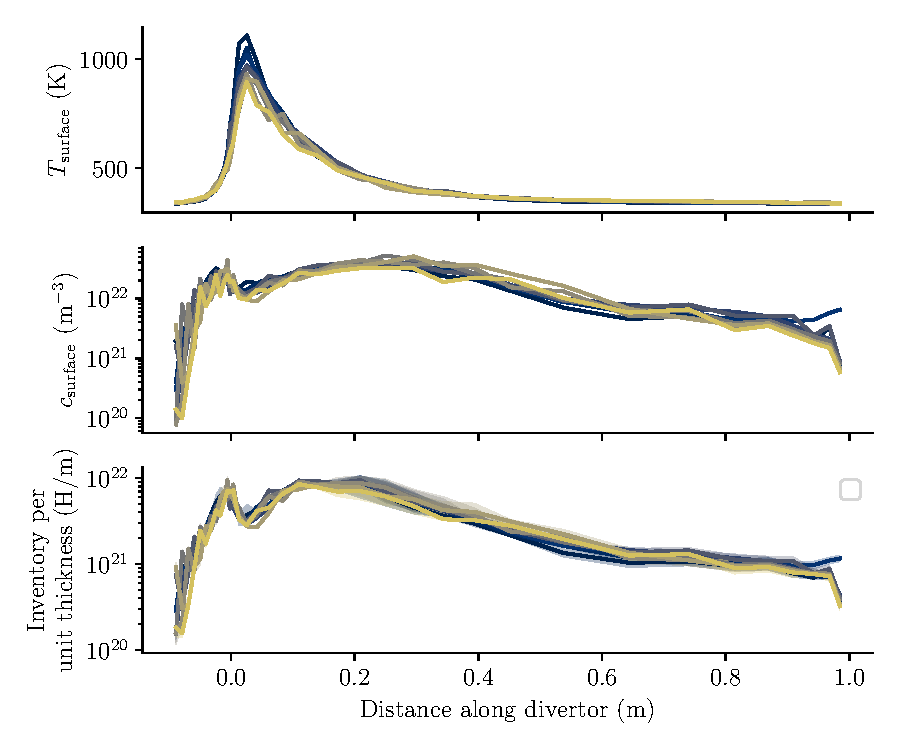
\includegraphics[width=\linewidth]{Figures/Chapter4/ITER/inventory_along_inner_divertor.pdf}
        \caption{IVT.}
    \end{subfigure}%
    \begin{subfigure}{0.58\linewidth}
        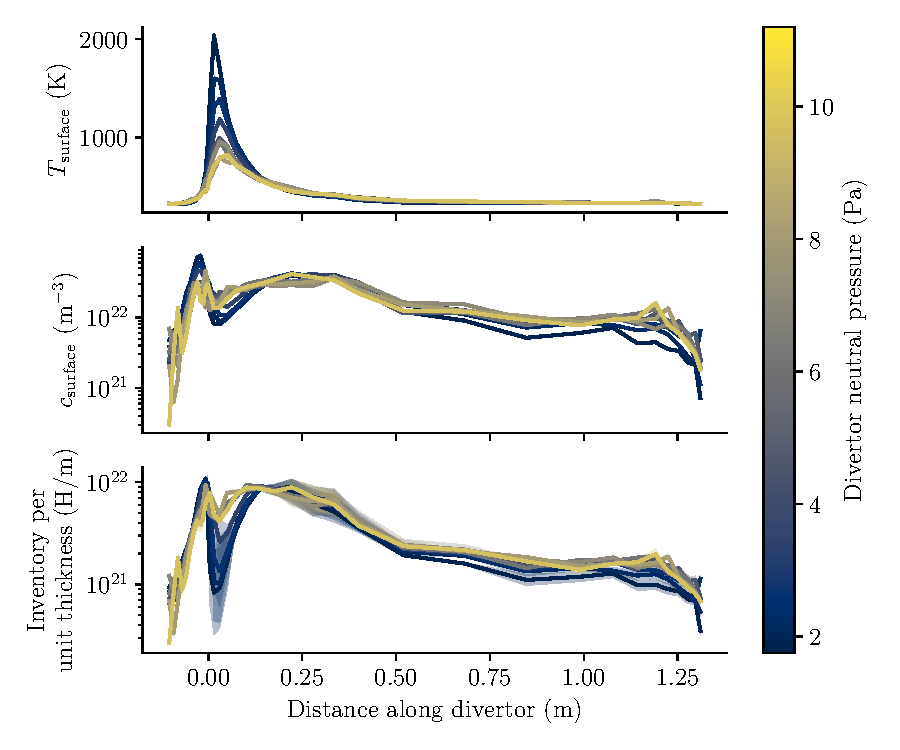
\includegraphics[width=\linewidth]{Figures/Chapter4/ITER/inventory_along_outer_divertor.pdf}
        \caption{OVT.}
        \labfig{distrib outer target}
    \end{subfigure}
    \caption{Surface temperature, surface concentration and inventory per unit thickness along the ITER divertor with neutral pressures varying from \SI{2}{Pa} to \SI{11}{Pa}. The area corresponds to the 95\% confidence interval.}
\end{figure*}


\begin{figure}[h]
    \centering
    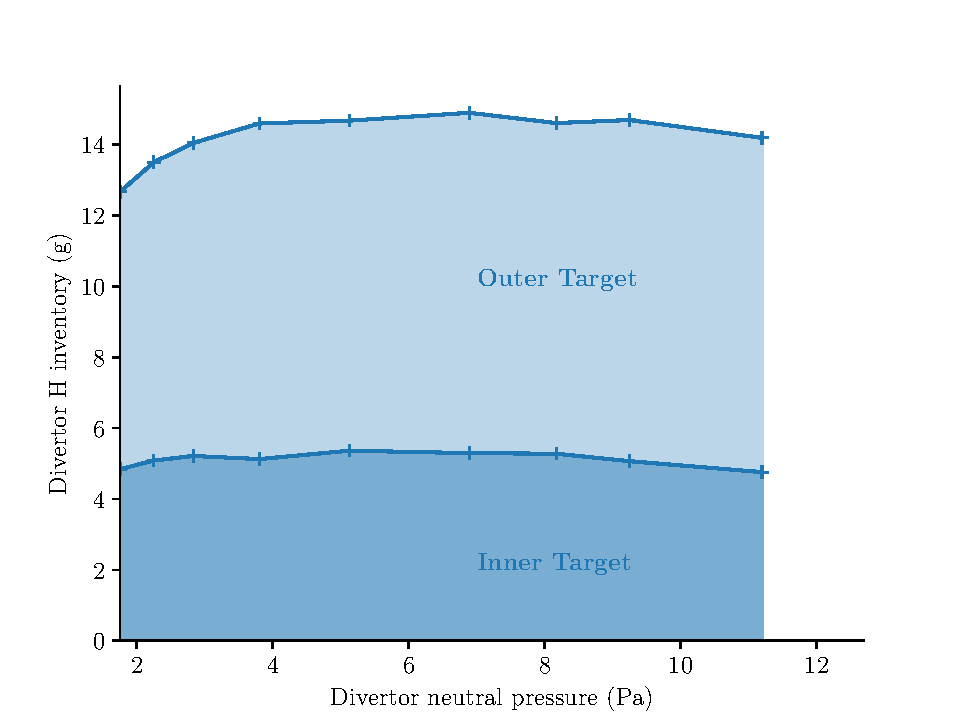
\includegraphics[width=\linewidth]{Figures/Chapter4/ITER/inventory_vs_divertor_pressure.pdf}
    \caption{Hydrogen inventory in the ITER divertor as a function of neutral pressure after \SI{e7}{s} of exposure (approximately 25 000 discharges).}
    \labfig{inventory vs neutral pressure}
\end{figure}


\begin{figure}[h!]
    \centering
    \begin{subfigure}{\linewidth}
        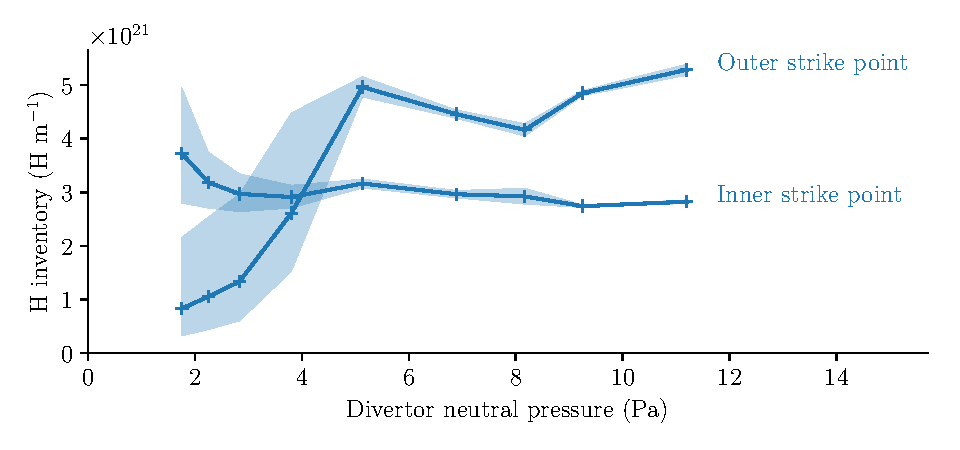
\includegraphics[width=\linewidth]{Figures/Chapter4/ITER/inventory_at_strike_points.pdf}
        \caption{Inventory per unit thickness after \SI{e7}{s} of exposure (approximately 25 000 discharges). Area corresponds to the 95\% confidence interval.}
        \labfig{local inventory neutral pressure}
    \end{subfigure}
    \begin{subfigure}{\linewidth}
        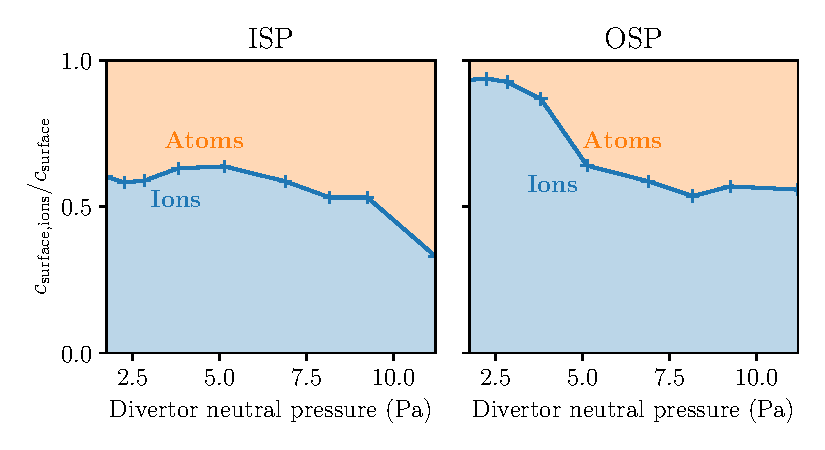
\includegraphics[width=\linewidth]{Figures/Chapter4/ITER/ratio_ions_atoms.pdf}
        \caption{Contribution of ions to the surface concentration of H.}
        \labfig{ion contribution neutral pressure}
    \end{subfigure}%
    \caption{H retention at the strike points (defined as maximum temperature) as a function of the divertor neutral pressure.}
\end{figure}

\begin{figure}[h!]
    \centering
    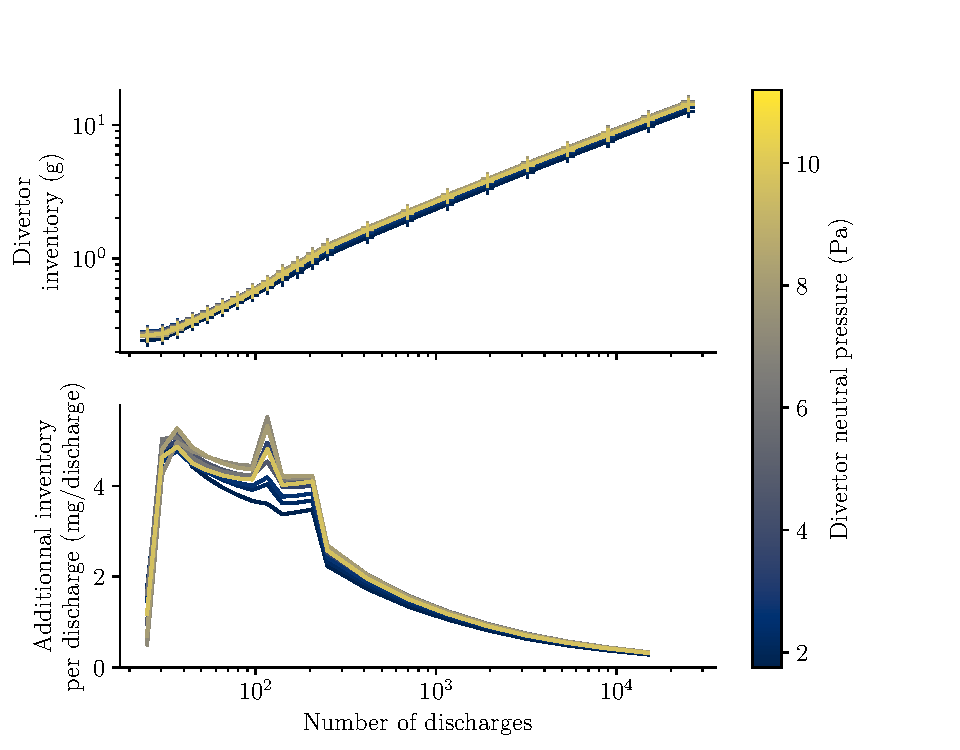
\includegraphics[width=\linewidth]{Figures/Chapter4/ITER/inventory_vs_time.pdf}
    \caption{Evolution of the H inventory of the ITER divertor with the number of \SI{400}{s} discharges.}
    \labfig{iter vs time}
\end{figure}


% peak temperature
Peak temperatures at strike points increased when decreasing the divertor neutral pressure (see \reffig{distrib outer target}).
The peak temperature at the outer strike point reached \SI{2000}{K} at \SI{2}{Pa} and more than \SI{1000}{K} at the inner strike point, which is in accordance with the results obtained by Pitts et al.\ \sidecite{pitts_physics_2019}.

% global inventory
The inventory in the whole divertor is computed as follows:
\begin{equation}
    \mathrm{inv_{divertor}} = N_\mathrm{cassettes} \cdot (\mathrm{inv_{IVT}} + \mathrm{inv_{OVT}})
\end{equation}
with $N_\mathrm{cassettes}=54$ the number of cassettes, $\mathrm{inv_{IVT}}$ and $\mathrm{inv_{OVT}}$ the total inventory in the IVT and OVT respectively (in one cassette).

\begin{align}
    \mathrm{inv_{IVT}} &= N_\mathrm{PFU-IVT} \cdot \int_\mathrm{IVT} \mathrm{inv_{MB}}(x)\: dx \\
    \mathrm{inv_{OVT}} &= N_\mathrm{PFU-OVT} \cdot \int_\mathrm{OVT} \mathrm{inv_{MB}}(x)\: dx
\end{align}
$N_\mathrm{PFU-IVT}=16$ and $N_\mathrm{PFU-OVT}=22$ the number of plasma facing units per cassette in the inner and outer targets respectively (see \refsec{divertor section}), $\mathrm{inv_{MB}}$ is the monoblock inventory per unit thickness and $x$ the distance along the targets.
Here, $\int_\mathrm{OVT} \mathrm{inv_{MB}}(x) dx$ corresponds to the area of the profile shown on \reffig{distrib outer target}.

The inventory in the outer target was found to be nearly twice that of the inner target.
This is largely explained by the larger number of plasma facing units in the outer target and therefore a greater exposed surface.
The global inventory increased with the divertor neutral pressure and a roll-over is observed above \SI{7}{Pa} (see \reffig{inventory vs neutral pressure}).
This roll-over is consistent with the results obtained in \sidecite{pitts_physics_2019}.
The inventory increase was found to be more important in the outer vertical target.
This was explained by the fact that the plasma is more detached at the inner target.
Therefore the surface temperature reduction is more significant in the outer vertical target and the surface concentration is increased (see \reffig{distrib outer target}).

The maximum inventory was found at around \SI{7}{Pa} and was approximately \SI{14}{g} of H, which is well below the ITER in-vessel safety limit of tritium (\SI{1}{kg}), especially considering only half of this quantity will be tritium.
This is especially true considering that this was for a very long exposure time of \SI{e7}{s}, which corresponds to 25 000 pulses of \SI{400}{s}.


% local inventories
The inventory at the inner and outer strike points globally increases with the divertor neutral pressure (see \reffig{local inventory neutral pressure}).
The contribution of ions to the surface concentration at the inner strike point is around 50 \% and tends to decrease with increasing neutral pressure (see \reffig{ion contribution neutral pressure}).
At low divertor neutral pressure, the contribution of ions at the outer strike point is around 90 \% and tends to decrease with increasing neutral pressure.
This can be explained by the fact that in both inner and outer targets, the integrated flux of ions decreases with increasing neutral pressure whereas the integrated flux of atoms increases, leading to a greater proportion of neutral particles.

% temporal evolution
For all divertor neutral pressures, the temporal evolution of the divertor inventory is approximately the same (see \reffig{iter vs time}).
The inventory is plotted as a function of the number of ITER discharges (see \reffig{plasma cycle}).
The additional inventory per \SI{400}{s} discharge was found to decrease with time.
Past 300 discharges, the additional inventory per discharge decreases with the number of discharges.
The maximum is around \SI{5}{mg/discharge} between 30 and 100 discharges.

\section{WEST results}

All the computations have been made for very long exposure times (\SI{e7}{s}) in order to better visualise trends.
Even though cycling can have an effect on H outgassing at the monoblock plasma facing surface, it was shown in \sidecite{hodille_modelling_2021} that the evolution of the monoblock inventory with the fluence was not affected.
Moreover, it can be shown that the divertors inventories evolve with a power law dependence of time.

\subsection{Influence of the input power}

The input power was varied between \SI{0.49}{MW} and \SI{2.0}{MW}.
Two puffing rate values were used: \SI{2.5e21}{molecule.s^{-1}} and \SI{4.4e21}{molecule.s^{-1}}.

\begin{figure}[h]
    \centering
    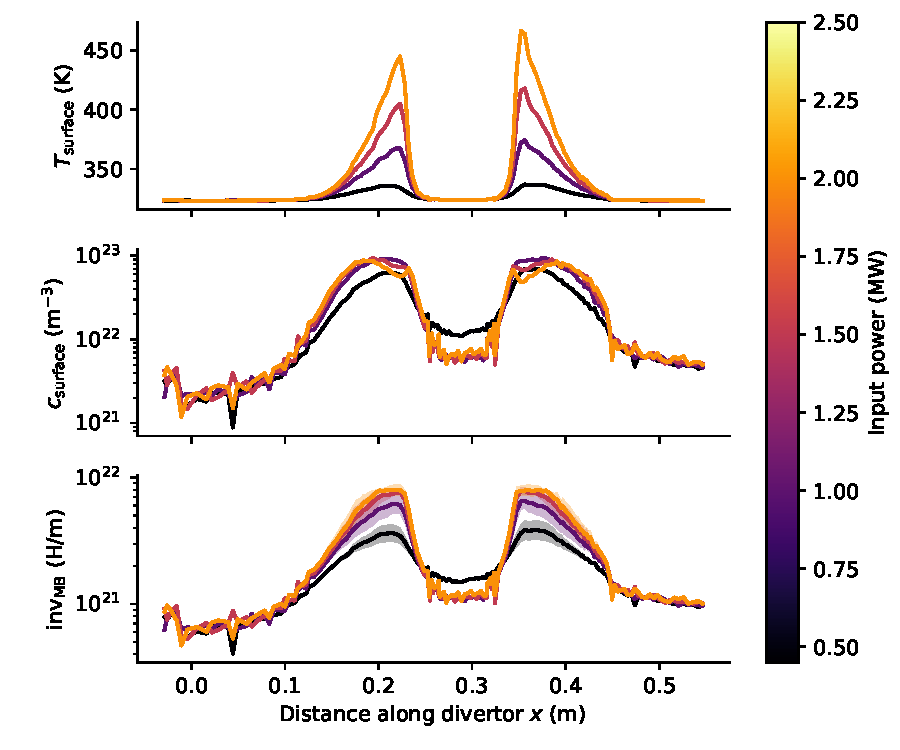
\includegraphics[width=\linewidth]{Figures/Chapter4/WEST/inventory_along_divertor_input_power.pdf}
    \caption{Distribution of surface temperature $T_\mathrm{surface}$, surface concentration $c_\mathrm{surface}$ and inventory per unit thickness along the WEST divertor with input powers varying from \SI{0.49}{MW} to \SI{2.0}{MW} with a puffing rate of \SI{2.5e21}{molecule.s^{-1}}.}
    \labfig{divertor distr power scan}
\end{figure}

\begin{figure}[h]
    \centering
    \begin{subfigure}{\linewidth}
        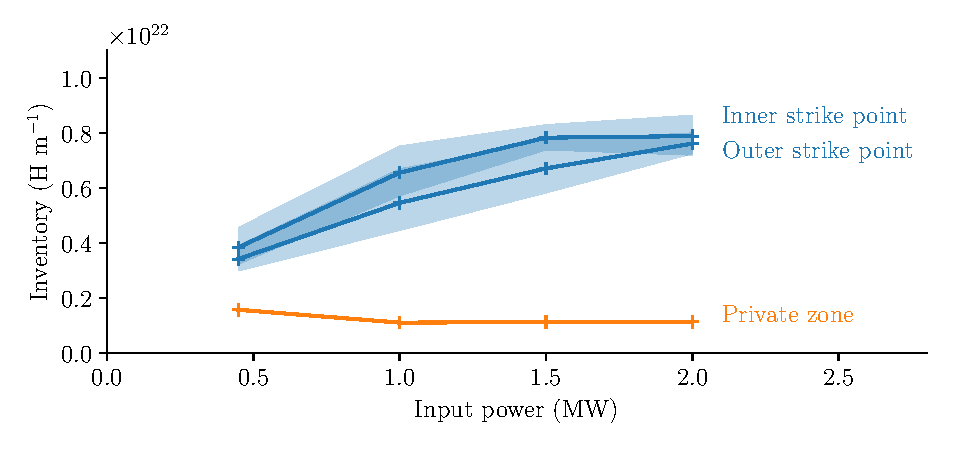
\includegraphics[width=\linewidth]{Figures/Chapter4/WEST/inventory_at_sps_and_private_zone_vs_input_power.pdf}
        \caption{Inventory per unit thickness after \SI{e7}{s} of exposure. The area corresponds to the 95\% confidence interval.}
        \labfig{local retention vs input power}
    \end{subfigure}
    \begin{subfigure}{\linewidth}                          
        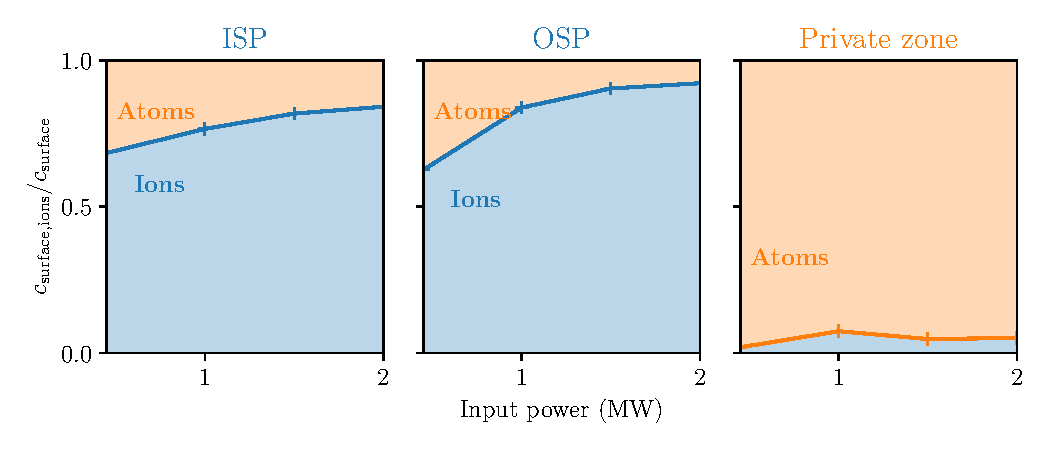
\includegraphics[width=\linewidth]{Figures/Chapter4/WEST/ions_ratio_vs_input_power.pdf}
        \caption{Contribution of ions to the surface concentration of H. ISP and OSP stand for Inner Strike Point and Outer Strike Point respectively.}
        \labfig{ion ration vs input power}
    \end{subfigure}%
    \caption{H inventory at the inner and outer strike points (ISP and OSP) and in the private zone as a function of the input power with a puffing rate of \SI{2.5e21}{molecule.s^{-1}}.}
\end{figure}

\begin{figure}
    \centering
    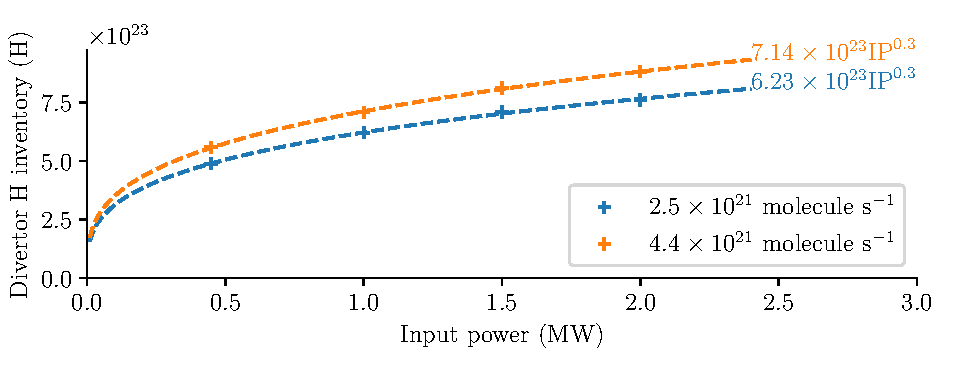
\includegraphics[width=\linewidth]{Figures/Chapter4/WEST/inventory_vs_input_power.pdf}
    \caption{Evolution of the WEST divertor inventory as a function of input power for several puffing rates.}
    \labfig{inventory vs input power}
\end{figure}

\begin{figure}[h]
    \centering
    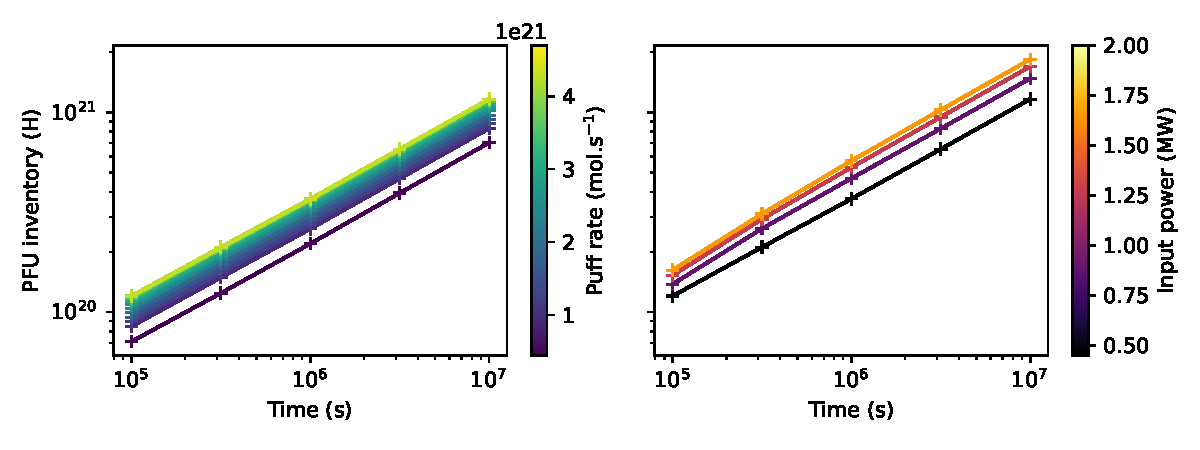
\includegraphics[width=\linewidth]{Figures/Chapter4/WEST/inventory_vs_time_west.pdf}
    \caption{Temporal evolution of PFU inventories for different values of puffing rate (left) and input power (right).}
    \labfig{temporal evolution west}
\end{figure}

% local inventories
The maximum retention was found to be located at the strike points (see \reffig{divertor distr power scan}).
The inventory at the outer strike point was higher than at the inner strike point.
The retention at the strike points was found to increase with the input power whereas it slightly decreased in the private zone (see \reffig{local retention vs input power}).
This was explained by an attachment of the plasma decreasing the particle flux in the private zone.
Since the surface temperature is constant, this leads to a decrease in the surface concentration of hydrogen as seen on \reffig{divertor distr power scan}.
On the other hand, the increasing temperature at the strike points only enhanced the diffusion process while remaining low enough so that hydrogen could get trapped.

The total inventory in the WEST divertor is computed as follows:
\begin{equation}
    \mathrm{inv}_\mathrm{divertor} = N_\mathrm{PFU} \cdot \int \mathrm{inv}_\mathrm{MB}(x)\: dx
    \labeq{inventory WEST}
\end{equation}
where $N_\mathrm{PFU} = 480$ is the number of PFU (Plasma Facing Units) in WEST, $\mathrm{inv}_\mathrm{MB}$ is the inventory per unit thickness in \si{H.m^{-1}} (see \reffig{divertor distr power scan}) and $x$ the distance along the target in \si{m}.

The divertor inventory increased with the input power (see \reffig{inventory vs input power}) and evolved as the power 0.3 of the input power.
The maximum divertor inventory was \SI{8.8e23}{H} at \SI{2.0}{MW} of input power.
This value of input power is still relatively low.
Increasing the puffing rate lead to an increase in the inventory.
This will be explained more thoroughly in \refsec{density scan}.

At the strike points, the retention is dominated by the ion flux whereas neutrals are dominant in the private zone (see \reffig{ion ration vs input power}).
The contribution of ions at the strike points increased with the input power but remained approximately constant in the private zone.

The divertor inventory was found to increase as a power law of time (see \reffig{temporal evolution west}).


\subsection{Influence of the puffing rate} \labsec{density scan}

A parametric study on the puffing rate was performed.
The puffing rate was varied between \SI{4.4e20}{molecule.s^{-1}} and \SI{4.7e21}{molecule.s^{-1}}.
The input power was fixed to \SI{0.45}{MW}.

\begin{figure}[h]
    \centering
    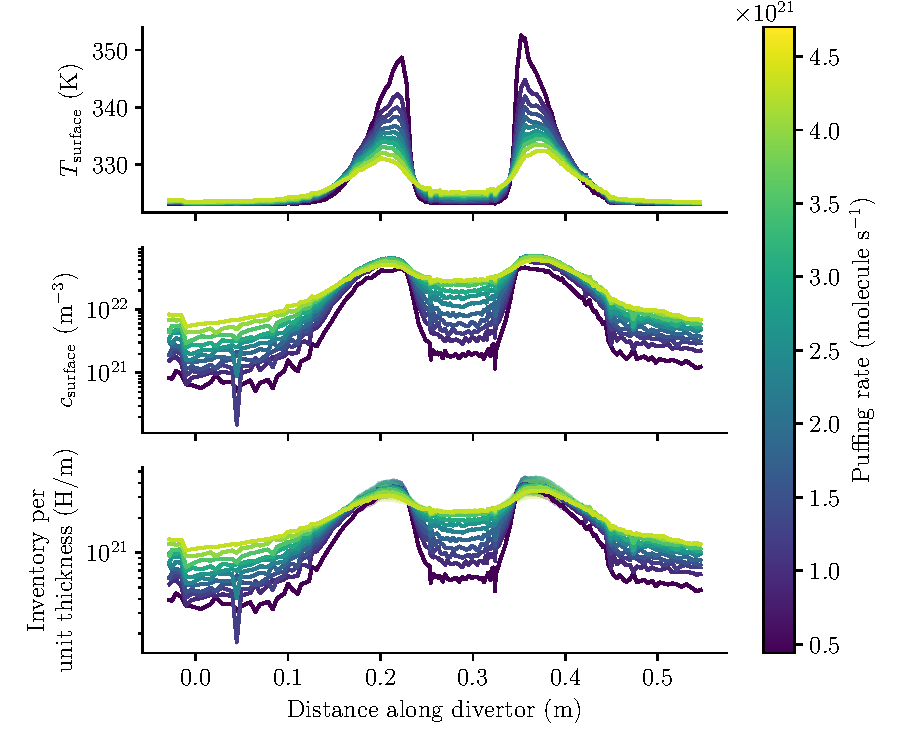
\includegraphics[width=\linewidth]{Figures/Chapter4/WEST/inventory_along_divertor.pdf}
    \caption{Distribution of surface temperature $T_\mathrm{surface}$, surface concentration $c_\mathrm{surface}$ and inventory per unit thickness along the WEST divertor with a puffing rate varying from \SI{4.4e20}{s^{-1}} to \SI{4.7e21}{s^{-1}} with \SI{0.45}{MW} of input power.}
    \labfig{divertor distr density scan}
\end{figure}

\begin{figure}[h]
    \centering
    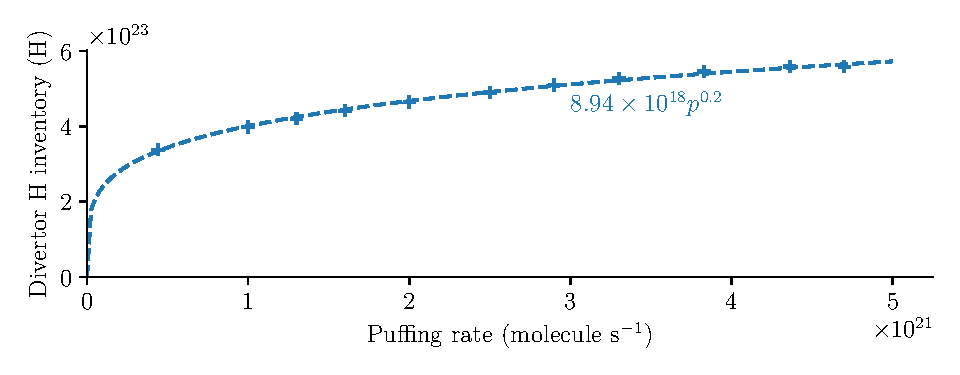
\includegraphics[width=\linewidth]{Figures/Chapter4/WEST/inventory_vs_puffing_rate.pdf}
    \caption{Evolution of the WEST divertor inventory as a function of puffing rate.}
    \labfig{inventory vs puffing rate}
\end{figure}

\begin{figure}[h!]
    \centering
    \begin{subfigure}{\linewidth}
        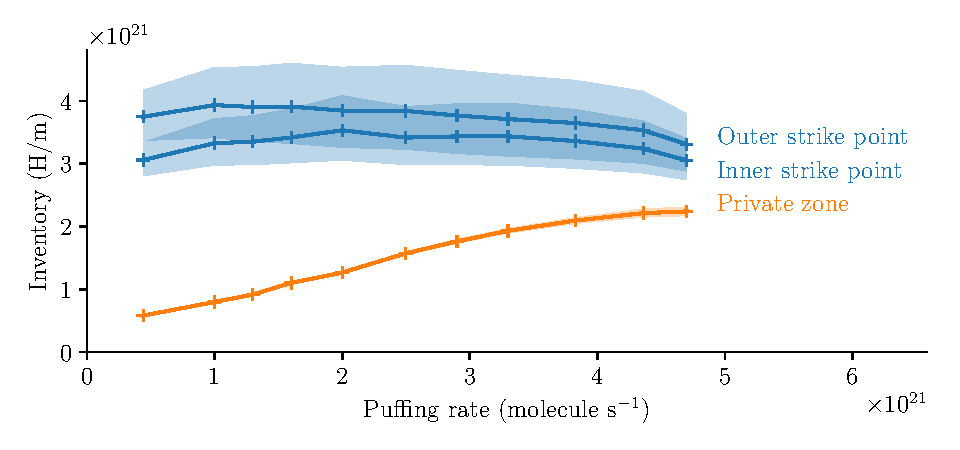
\includegraphics[width=\linewidth]{Figures/Chapter4/WEST/inventory_at_sp_and_private_zone.pdf}
        \caption{Inventory per unit thickness after \SI{e7}{s} of exposure. The area corresponds to the 95\% confidence interval.}
        \labfig{local retention vs puffing rate}
    \end{subfigure}
    \begin{subfigure}{\linewidth}
        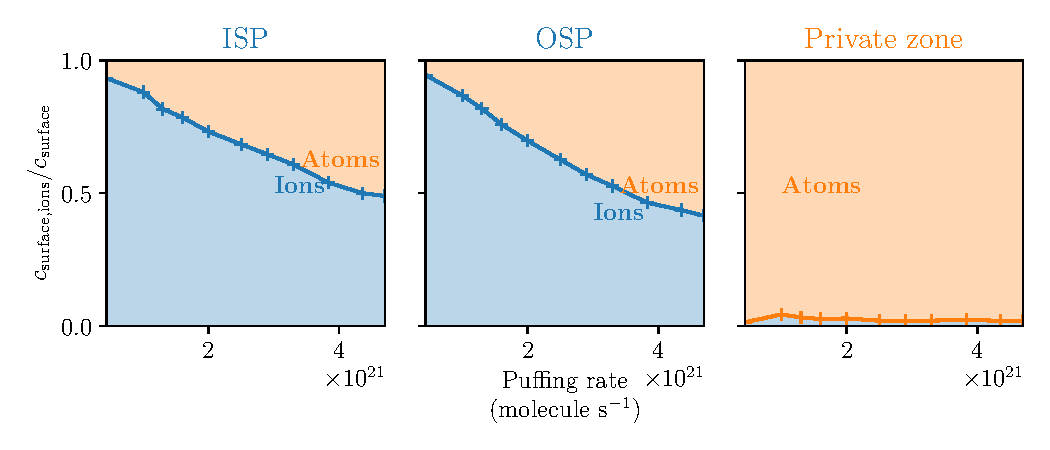
\includegraphics[width=\linewidth]{Figures/Chapter4/WEST/ion_ratio_at_sp_and_private_zone.pdf}
        \caption{Contribution of ions to the surface concentration of H. ISP and OSP stand for Inner Strike Point and Outer Strike Point respectively.}
        \labfig{ion contribution vs puffing rate}
    \end{subfigure}%
    \caption{H retention at the strike points and in the private zone as a function of puffing rate with \SI{0.45}{MW} of input power.}
\end{figure}

The maximum retention was again located at the strike points for all puffing rates values (see \reffig{divertor distr density scan}).
The inventory at the outer strike point was higher than at the inner strike point.
The inventory in the private zone was found to increase with the puffing rate whereas it was almost constant at the strike points (see \reffig{local retention vs puffing rate}).
As for the power scan, the ions' contribution to the inventory is rather low in the private zone (see \reffig{ion contribution vs puffing rate}).
Moreover, the contribution of ions decreases rapidly at the strike points and represents only half of the surface concentration at \SI{4e21}{molecule.s^{-1}}.

The inventory in the whole WEST divertor is computed from \refeq{inventory WEST}.
As for the power scan, the divertor inventory increased as the power 0.2 of the puffing rate (see \reffig{inventory vs puffing rate}).
The maximum inventory was found to be \SI{5e23}{H} at \SI{4.7e21}{molecule.s^{-1}}.

The divertor inventory was found to increase as a power law of time.

\section{Summary}


The monoblock behaviour law proposed in \refch{Chapter3} was used to estimate fuel retention in the divertors of WEST and ITER.
Key control parameters were investigated: the input power, the puffing rate and the divertor neutral pressure.
Their impact on the divertor inventory was studied.

It was shown that the inventory in WEST increases as the power $0.3$ of the input power and as the power $0.2$ of the puffing rate.
The inventory in the ITER divertor was found to first increase with the neutral pressure up to \SI{7}{Pa} then decrease, though the variation was smoother.
The inventory in the outer vertical target of the ITER divertor is twice that of the inner vertical target.
These results were in good agreement with the observations made in \sidecite{pitts_physics_2019}.

However, it should be noted that both machines do not operate in the same regime.
While WEST operates at low input power, ITER operates at high input power with a high recycling divertor.
These differences in the operation regime can explain different trends.

The maximum hydrogen inventory in the ITER divertor was approximately \SI{14}{g} after \SI{e7}{s} of continuous plasma exposure (25 000 ITER discharges), which is well below the safety limit (\SI{1}{kg}).
Moreover, since the behaviour law is based on 2D monoblock simulations, this value is an upper estimate.
2D simulations are indeed conservative in terms of inventory (see \refsec{influence of dimensionality}).

The underlying monoblock model has also a few limitations, as detailed in \refch{Chapter3}.
First, the set of trapping parameters that was used may not be relevant for every region of the divertor.
These properties can however be experimentally estimated.
The accuracy of the results could therefore be improved by running a new batch of FESTIM monoblock simulations with different trapping parameters like neutron-induced traps.

Then, this model does not take into account retention in Be co-deposited layers.
These are expected to be the main driver for H retention in ITER \sidecite{de_temmerman_data_2021}.
However, this work is still relevant for full-W environments like WEST or DEMO.
